\chapter{Diples}
\label{ch:diples}
\index{dessert}
\index{honey}
\index{Christmas}
\textit{Greek honey dipped fried pastries}

Family member: Grandma Elisavet

\marginnote[20pt]{\\
    \textbf{Makes 12+ servings} \\
    Prep time: 45 minutes \\
    Cook time: 1 hour \\
    \vspace*{\baselineskip}

    4 eggs \\
    4 small water glasses of sugar \\
    Flour, all-purpose, as much as the dough takes \\
    Greek honey \\
    Walnuts, crushed \\
    Cinnamon \\
    \vspace*{\baselineskip}

}
\newthought{Every Christmas} my grandma would make \textgreek{δίπλες}. A traditional Greek dessert from the Peloponnessos, diples are light and airy fried dough dipped in honey, walnuts and dusted with cinnamon. They can be kept for 1-2 weeks in a plastic container, lined with plastic wrap.

\begin{enumerate}
    \item In a large bowl, mix the eggs with the sugar. 
    \item Add flour, and mix until you can form a dough, mix slowly. If too stiff, add water bit by bit. If too soft, add some flour.
    \item Using a rolling pin, roll out the dough until you have thin sheets. Cut them into strips, then rectangles.
    \item Heat oil in a frying pan. One by one, fry the dough sheets. When they start to puff up, use a fork to roll them and form a cylinder. Once they start to color, remove them onto a plate lined with paper.
    \item Warm honey in a small pot. Once the diples have cooled down, drizzle some honey on top, add crushed walnuts and a sprinkle of cinnamon. Serve with coffee after Christmas dinner!
\end{enumerate}

\begin{marginfigure}
  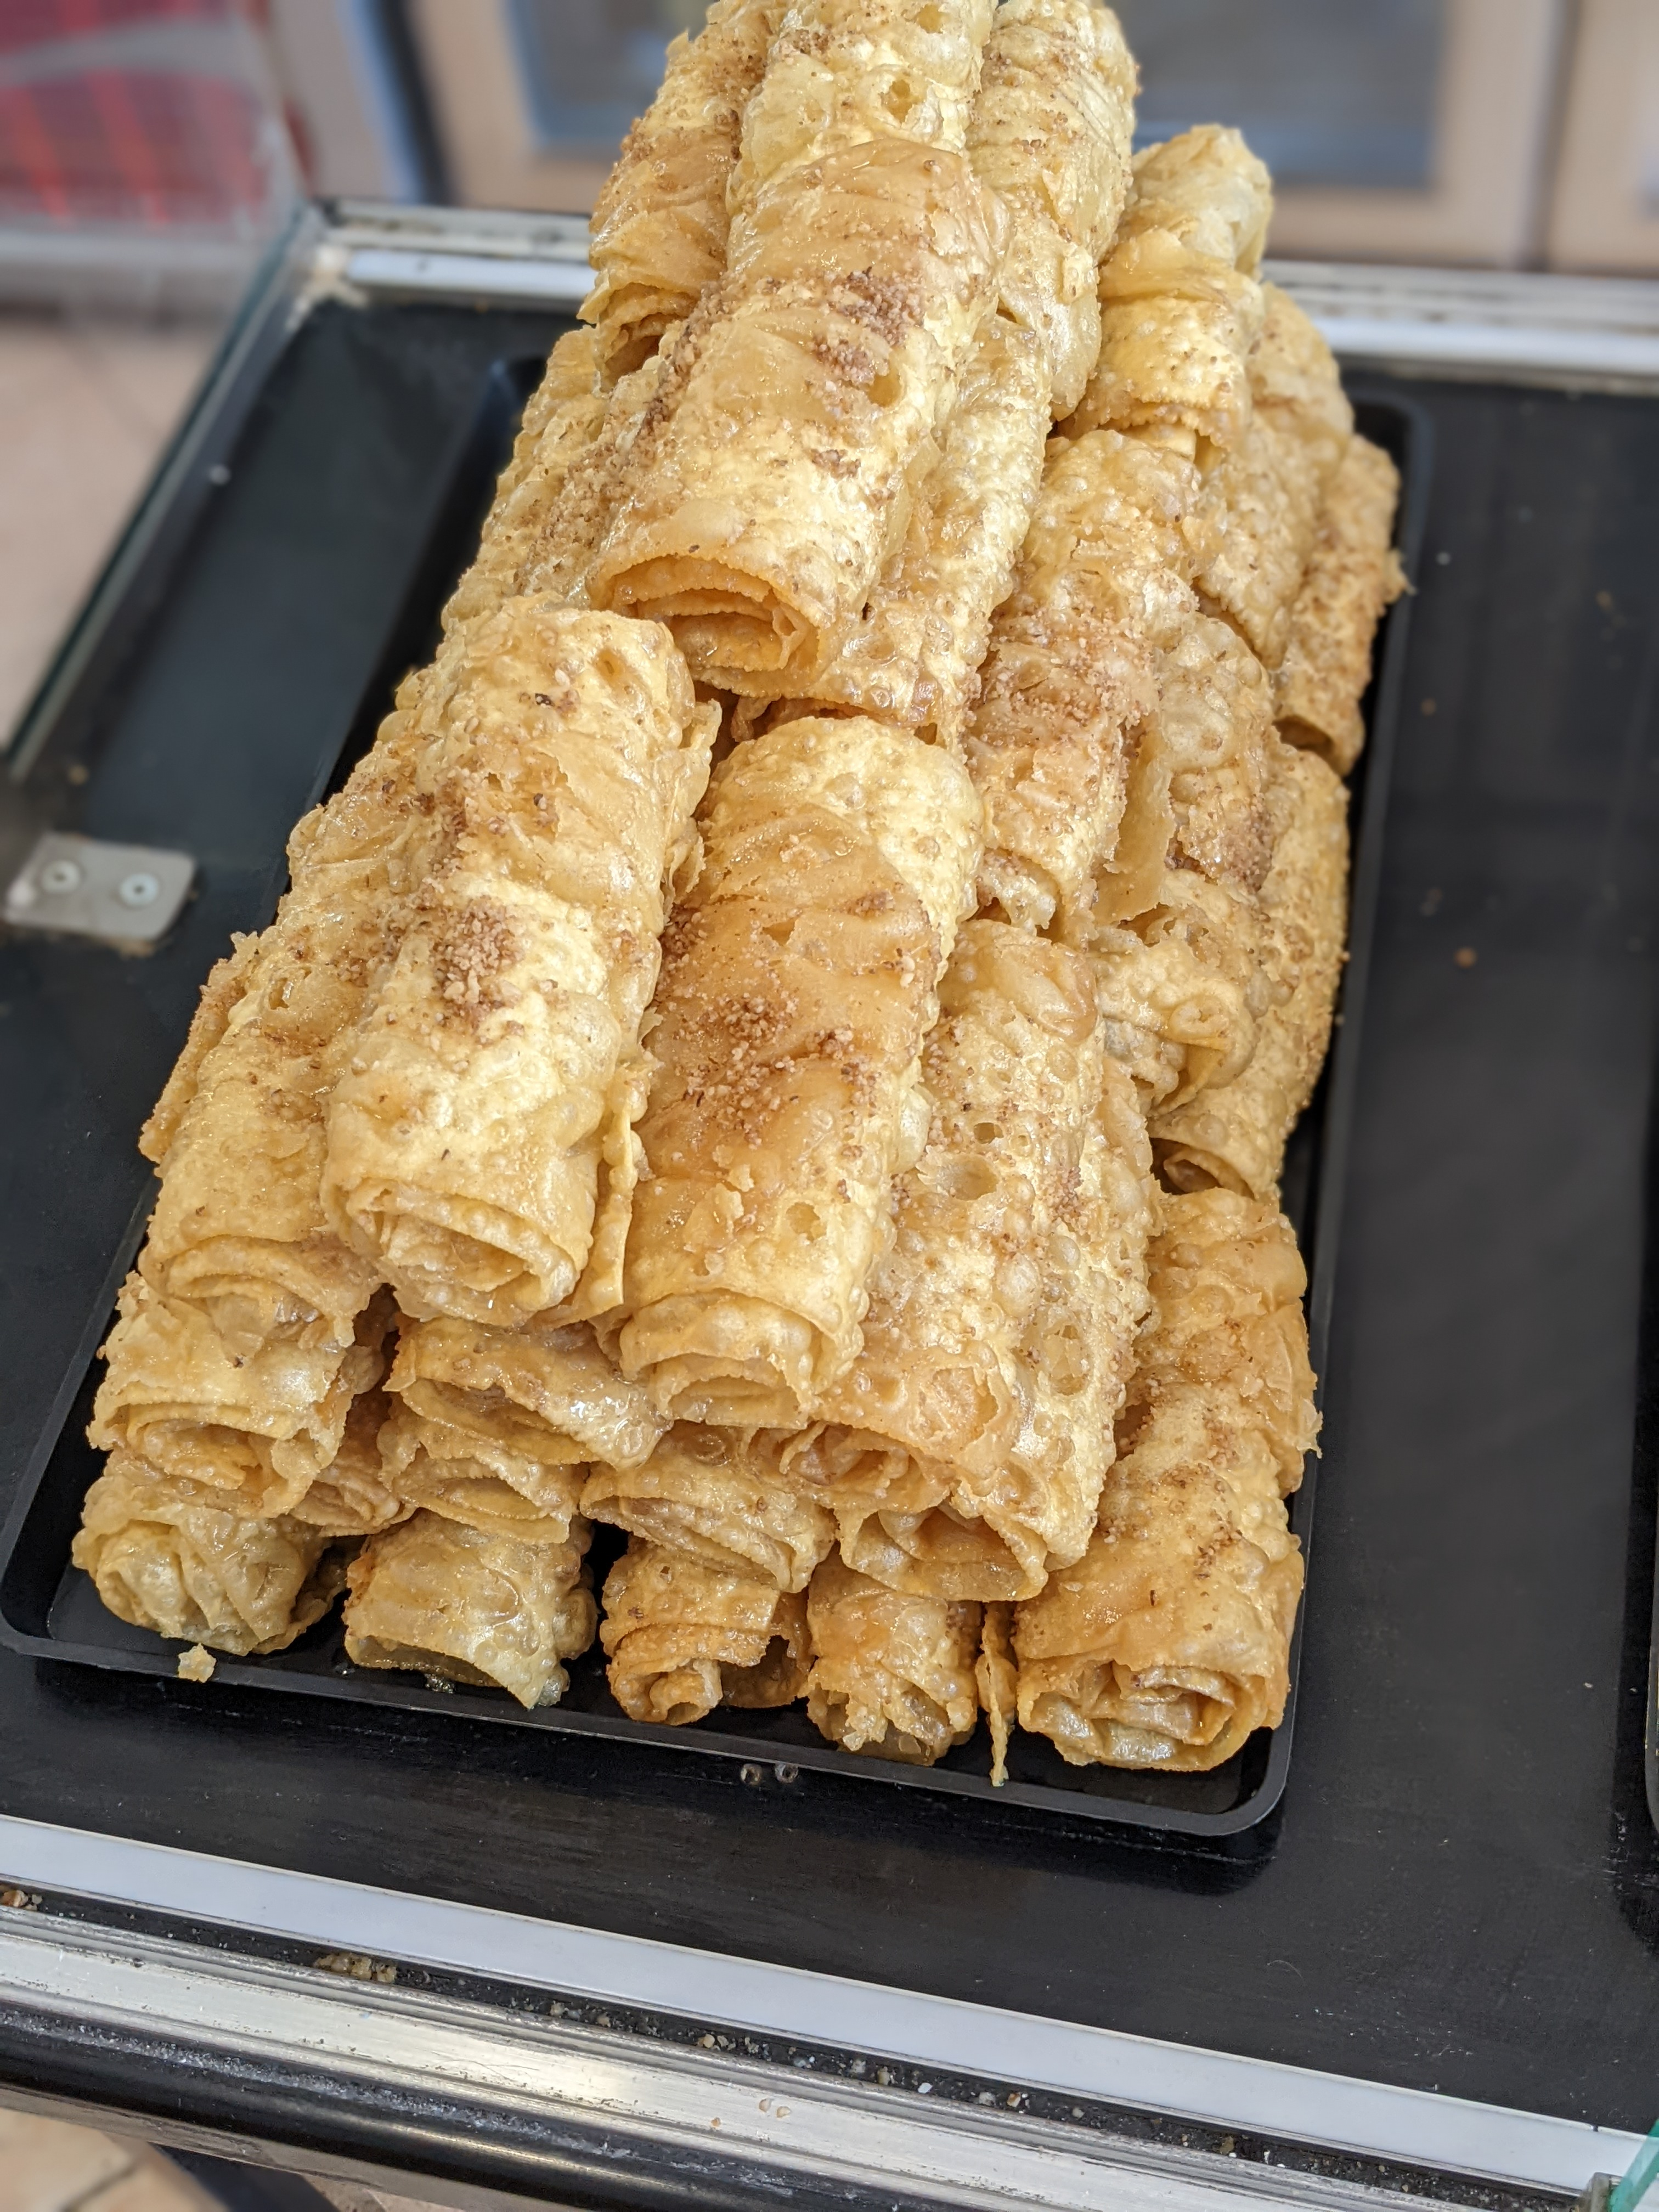
\includegraphics[width=60mm]{monanteras/images/Diples.jpg}
  \caption{Diples from a bakery in the town of Levidi, Arcadia}
\end{marginfigure}
